\section{Experiences and Numerical Analysis}

\subsection{Analysis of the ascent step convergence}

 During the iterative procedure, we plot the evolution of the converge criteria, namely $\norm{ \frac{\partial F}{\partial \phi_j} }$ for $j \in \intinter{1}{J}$. 
\begin{figure}
    \begin{subfigure}{.5\textwidth}
        \centering
        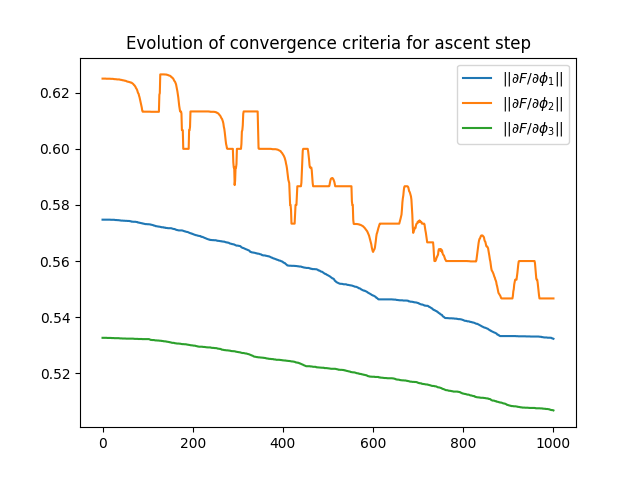
\includegraphics[width=\textwidth]{figures/ascent_criteria_n_samples16000.png}
    \end{subfigure}
    \begin{subfigure}{.5\textwidth}
        \centering
        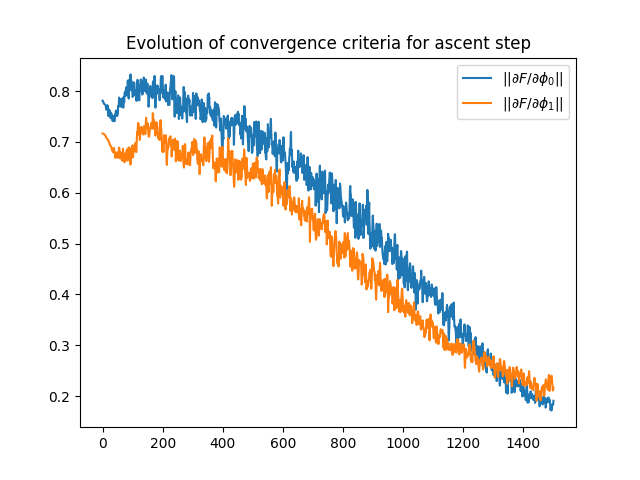
\includegraphics[width=\textwidth]{figures/ascent_criteria_msamples16000_iter0_1D_2skewnorm.png}
    \end{subfigure}
\end{figure}

The majority of computation time is consumed by the ascent step (~1 hours). 

The ascent step take most of the computation time. In \cite{claici_stochastic_2018}, the authors use a step size of $\alpha = 10^{-3}$ $\epsilon_{ascent} = 10^{-6}$ in Algorithm \ref{ascent}. However, the while loop took an excessive amount of time to converge, exceeding $4$ hours. To enhance computational efficiency, we opt for $\alpha = 0.05$ and $\epsilon_{ascent} = 10^{-4}$. Nesterov acceleration is set to $\beta = 0.99$ like in \cite{claici_stochastic_2018}. Additionally, we introduce a maximum number of iterations, limiting the while loop to $T_{max} = 1500$ for efficiency.


\subsection{Quantitative Analysis and Comparative Evaluation}

\subsubsection{Optimal Monge Map Approach to Barycenter Computation}
\label{sec:monge_map}

In the case $\mathcal{X} = \mathcal{Y} = \RR^d$ and $d(x, y)^2 = \norm{x  - y}^2$ and if at least one of the two input measures has a density with respect to the Lebesgue measure, the Theorem $2.1$ of \cite{peyre_computational_2020} states that the optimal coupling $\pi$ of \eqref{eq:W2} is unique and is given by $\pi = (Id, T)_\#\mu$ where $T : \mathcal{X} \rightarrow \mathcal{Y}$ denote the "optimal Monge map" with $T_\#\mu = \nu$. 

In the 1D case \cite[see][Remark 2.30]{peyre_computational_2020}, $d=1$, the optimal Monge map between two distributions $\mu_1$ and $\mu_2$ writes 

\begin{equation}\label{eq:monge_map}
    T=\mathcal{C}^{-1}_{\mu_2}\ o\ \mathcal{C}_{\mu_1} 
\end{equation}

where $\mathcal{C}_{\mu} : \RR \rightarrow [0, 1]$ and $\mathcal{C}^{-1}_\mu : [0, 1]\rightarrow \RR $ are respectively the cumulative distribution function and its pseudoinverse, also called the generalized quantile function of $\mu$ .

Using the Remark $7.1$ \cite{peyre_computational_2020}, the McCann's interpolation \cite{mccann_convexity_1997} between two measures reads, for $t\in [0, 1]$ 
\begin{align}
    \mu_t &= (tT + (1-t)Id)_\#\mu_1 \nonumber \\
    \mu_t &= (t\mathcal{C}^{-1}_{\mu_2}\ o\ \mathcal{C}_{\mu_1} + (1-t)Id)_\#\mu_1 \label{eq:mccann}
\end{align}

Figure \ref{fig:mccann_1D_2skew} shows the displacement interpolation between 1-D measures, using the cumulative distribution function as detailed in \eqref{eq:mccann}.

\begin{figure}[H]
    \centering
    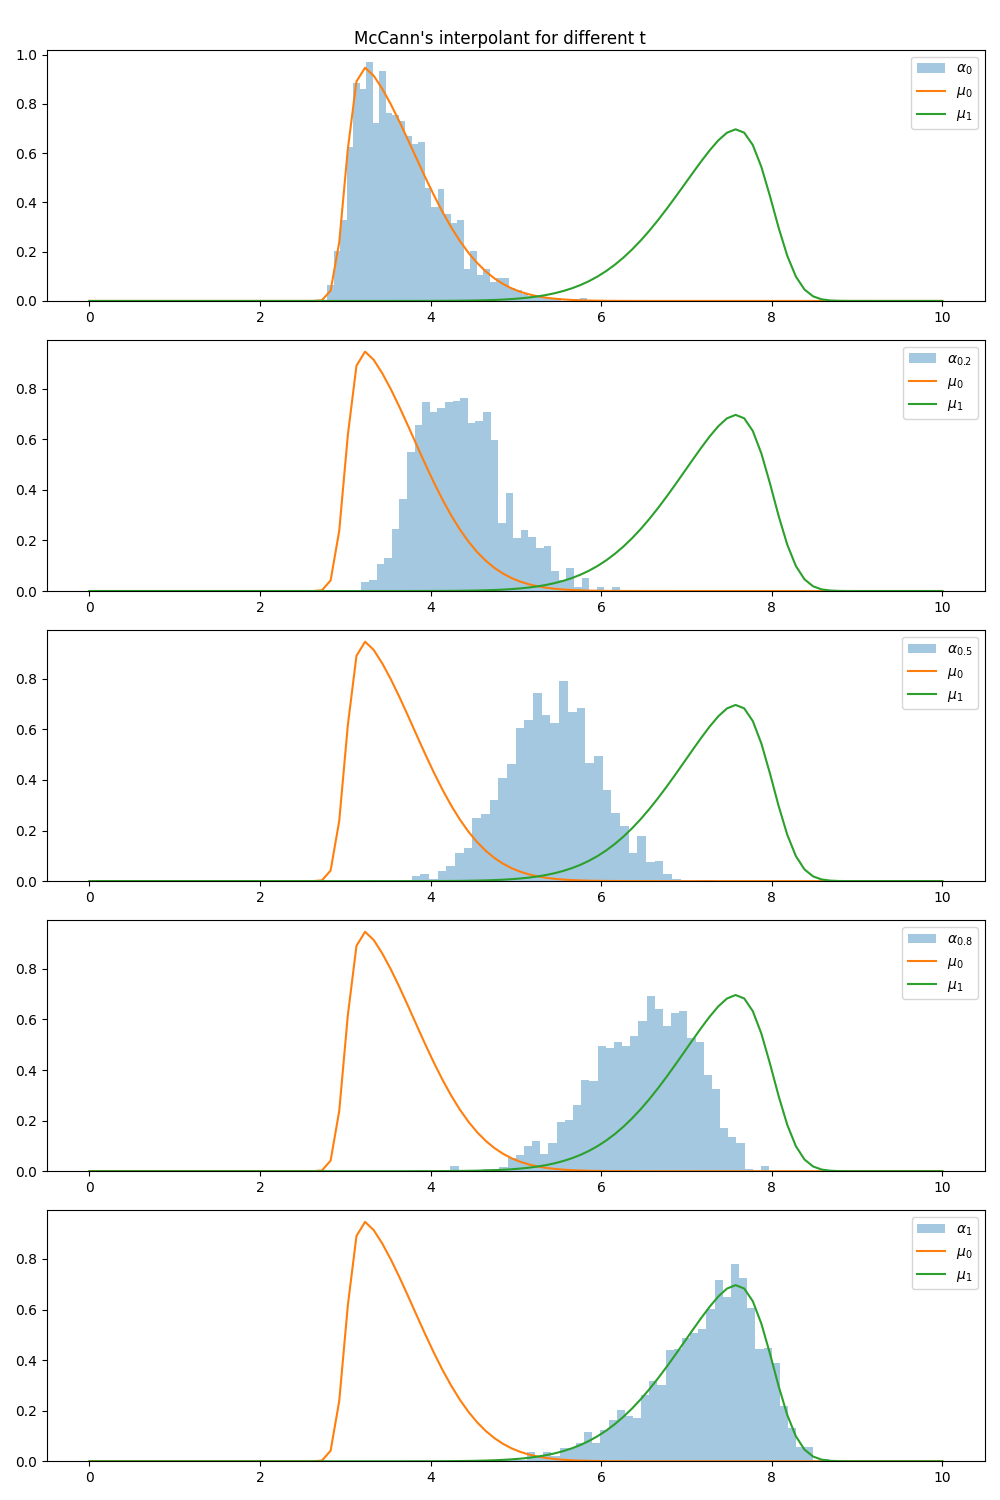
\includegraphics[width=\textwidth]{figures/mccann_1D_2skew.png}
    \caption{McCann's interpolant between two skew-normal distributions. From top to bottom, $t$=0, 0.2, 0.5, 0.8, 1.}
    \label{fig:mccann_1D_2skew}
\end{figure}

To obtain the interpolant, we generate $K$ samples $(X_k)$ independent and identically distributed (iid) according to $\mu_1$. Then, we compute the samples $(Y_k)$ as follows 
$$Y_k = tT X_k + (1-t)X_k, \qquad \forall k \in\intinter{1}{K}$$ 
where $T$ is given in \eqref{eq:monge_map}. We have that $ (Y_k)$ is iid according to $\mu_t$.

To compare with the algorithm \ref{ascent_snap}, we use $t=0.5$. The only hyperparameter to fix is the number of samples $K$ to generate. We choose $K=2000$. The inconvenient is that we can apply this computation only in the 1-D case and for two input measures.

\subsubsection{Computation of the barycenter with Iterative Bregman Projections} \label{sec:iterative_bregman}

We will also compare our algorithm \ref{ascent_snap} to the computation of the barycenter using the Sinkhorn algorithm \cite{peyre_computational_2020}. This algorithm solved the discretized regurlarized optimal transport problem using the optimality condition that shows that the optimal coupling $P_\epsilon$ necessarily has the form 
$$P_\epsilon = diag\left(u\right) K\ diag\left(v\right)$$
where the Gibbs kernel is defined as
$$K := e^{-\frac{C}{\epsilon}}.$$
where $C_{ij} = d(x_i, y_j)^2$ is the cost matrix. The vectors $u$ and $v$ are non negative vectors. $\epsilon$ is the regularization parameter.

Figure \ref{fig:sinkhorn_1D_2skew} depicts the barycenter obtained for various $\epsilon$. It's worth noting that the algorithm encounters instability issues for $\epsilon$ values below $0.005$. As illustrated, the lower $\epsilon$, the sharper the density of the barycenter.

\begin{figure}
    \centering
    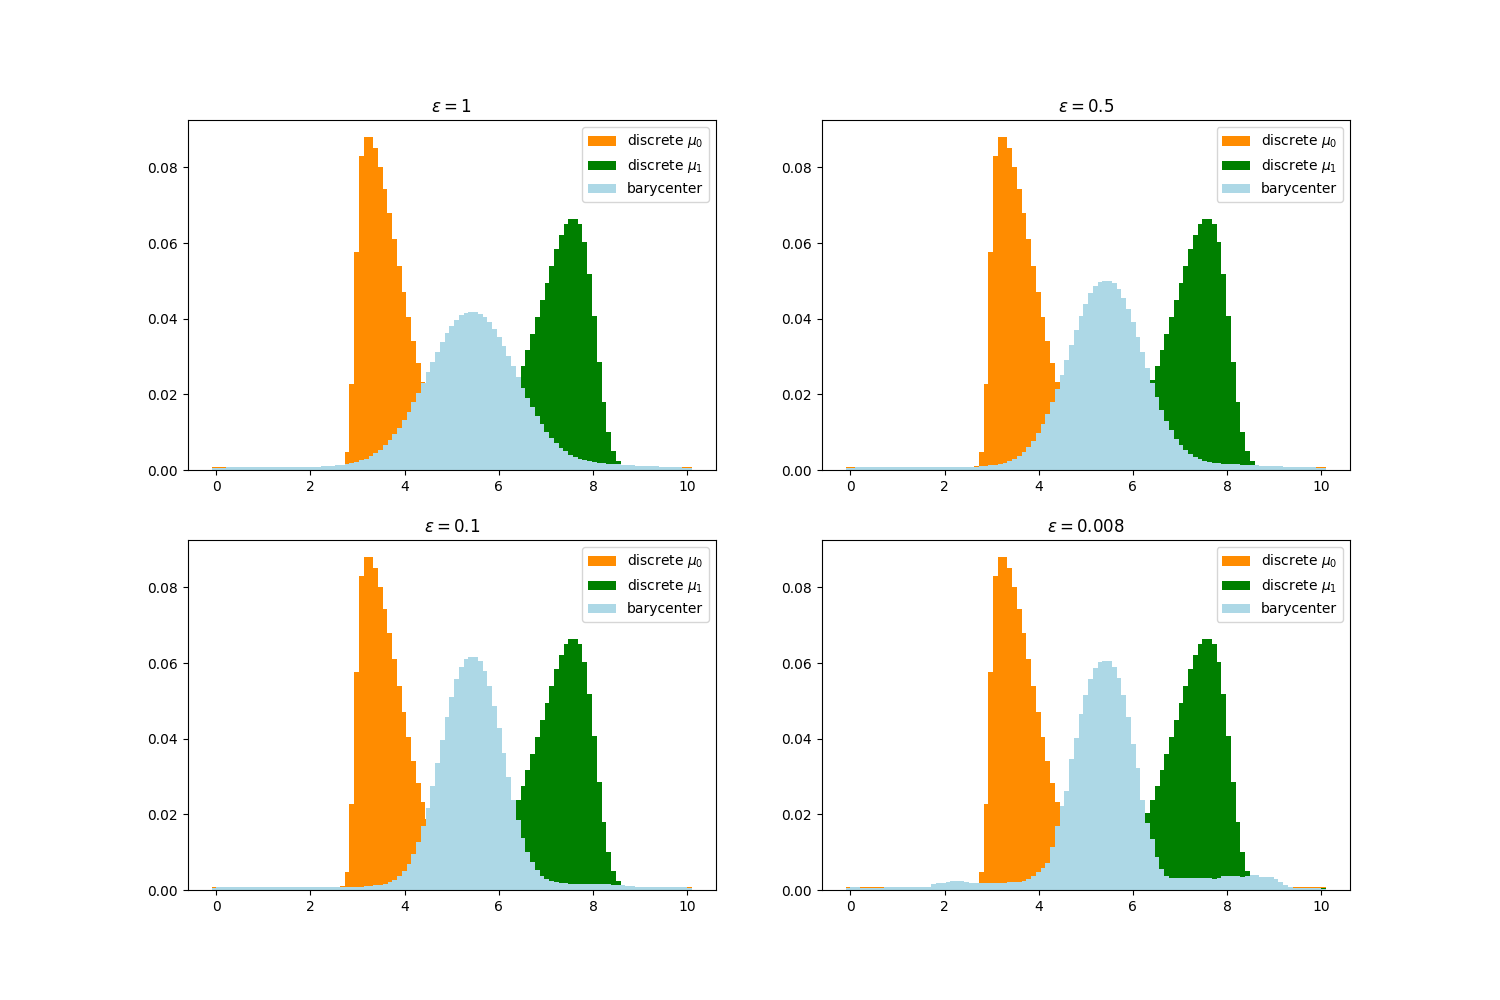
\includegraphics[width=\textwidth]{figures/sinkhorn_1D_2skew.png}
    \caption{Histogram showing the input distributions (skew-normal distributions) and the barycenter computed using the Sinkhorn algorithm for different values of the regurlarized parameter $\epsilon$.}
    \label{fig:sinkhorn_1D_2skew}
\end{figure}

Henceforth, we will use $\epsilon = 0.01$. 

\subsubsection{Computation on free grid using POT toolbox}

The POT toolbox (Python Optimal Transport) \cite{flamary_pot_2021} contains implementations of a number of founding works of OT for machine learning such as Sinkhorn algorithm and Wasserstein barycenters. In particular, it provides an algorithm based on \cite{cuturi_fast_2014} (Algorithm 2) that solves the free support regularized Wasserstein barycenter problem. Like the method \S\ref{sec:method}, we optimize over the locations of the barycenter but not over its weights. 

The figures \ref{pot1}, \ref{pot2} and \ref{pot3} in the Appendices shows the influence of the regularization $\epsilon$ on the free support barycenters for the 2D dataset.

\subsubsection{Experience 1 : 1D skewed normal distributions}

\subsubsection{Experience 2 : 2D uniform distributions}
